%!TEX root = thesis.tex
\chapter{Results}
\label{ch:results}

Optimum angles and their corresponding electricity use were found for the building energy simulation for all hours of the year. For the radiation and PV evaluations, a grid-convergence study was performed and results of an optimizing angle strategy was compared to sun-tracking. The combined simulations could then be evaluated to find the most efficient overall combinations and the sensitivities of various parameters on the system performance was found.

\section{Building Energy Analysis}
	
	The optimal configurations of the ASF can be visualised using carpet-plots. For a classical building analysis this was done for every hour of the year. Figures \ref{f:DIVAx} and \ref{f:DIVAy} show the optimizing altitude and azimuth angles for heating, cooling, lighting and total building energy demand. In figure \ref{f:DIVAx}, darker colours represent closed positions, whereas brighter colours correspond to open positions. To optimize heating and lighting, open positions (corresponding to large altitude angles) are favourable, cooling is optimized by using closed positions (corresponding to small altitude angles). The overall optimized solutions follow the corresponding patterns at the hours of importance. The azimuth angles in figure \ref{f:DIVAy} correspond to the deviation from the facade normal. For a south facing facade, this means an angle with a positive sign represents the panels facing towards south-east (bright colours), whereas negative angles represent the panels facing towards south-west (dark colours). It can be seen that for heating and lighting, the facade takes positions that let the sun in, whereas for cooling the facade follows a sun-tracking pattern which prevents radiation to enter the room. 

	\begin{figure*}
		\begin{center}
		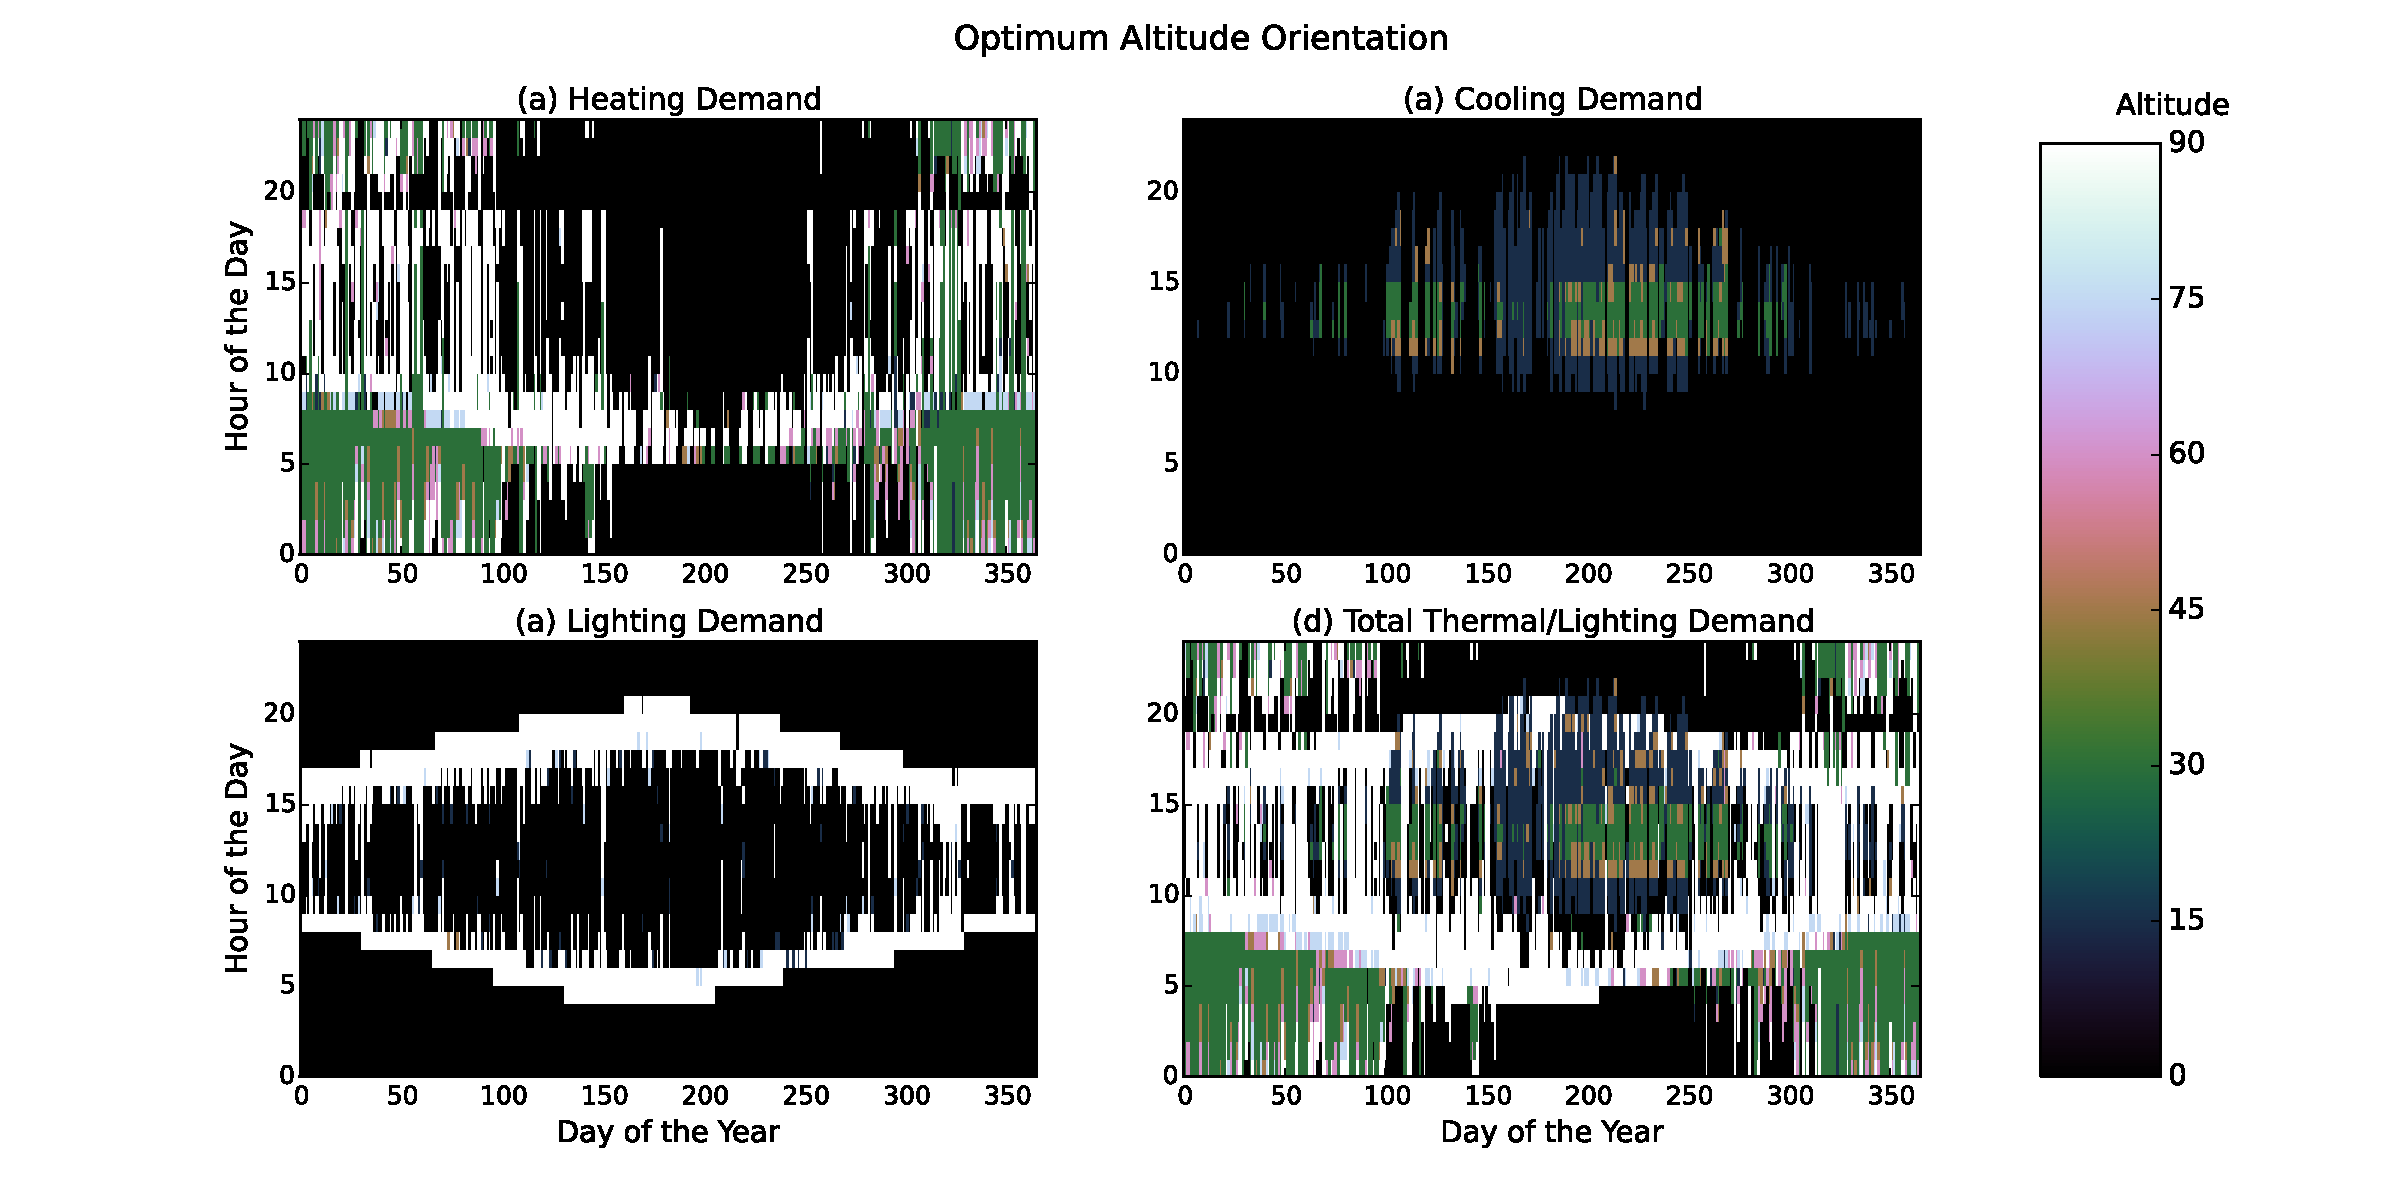
\includegraphics[width=\textwidth, trim= 0cm 0cm 0cm 0cm,clip]{DIVAx}
		\caption{Carpet plots detailing the optimal altitude angles to minimise the (a) heating demand, (b) cooling demand, (c) lighting demand, and (d) total building energy demand. Darker colours represent closed positions, whereas brighter colors correspond to open positions. To optimize heating and lighting, open positions are favorable, cooling is optimized by using closed positions.}
		\label{f:DIVAx}
		\end{center}
	\end{figure*}


	\begin{figure*}
		\begin{center}
		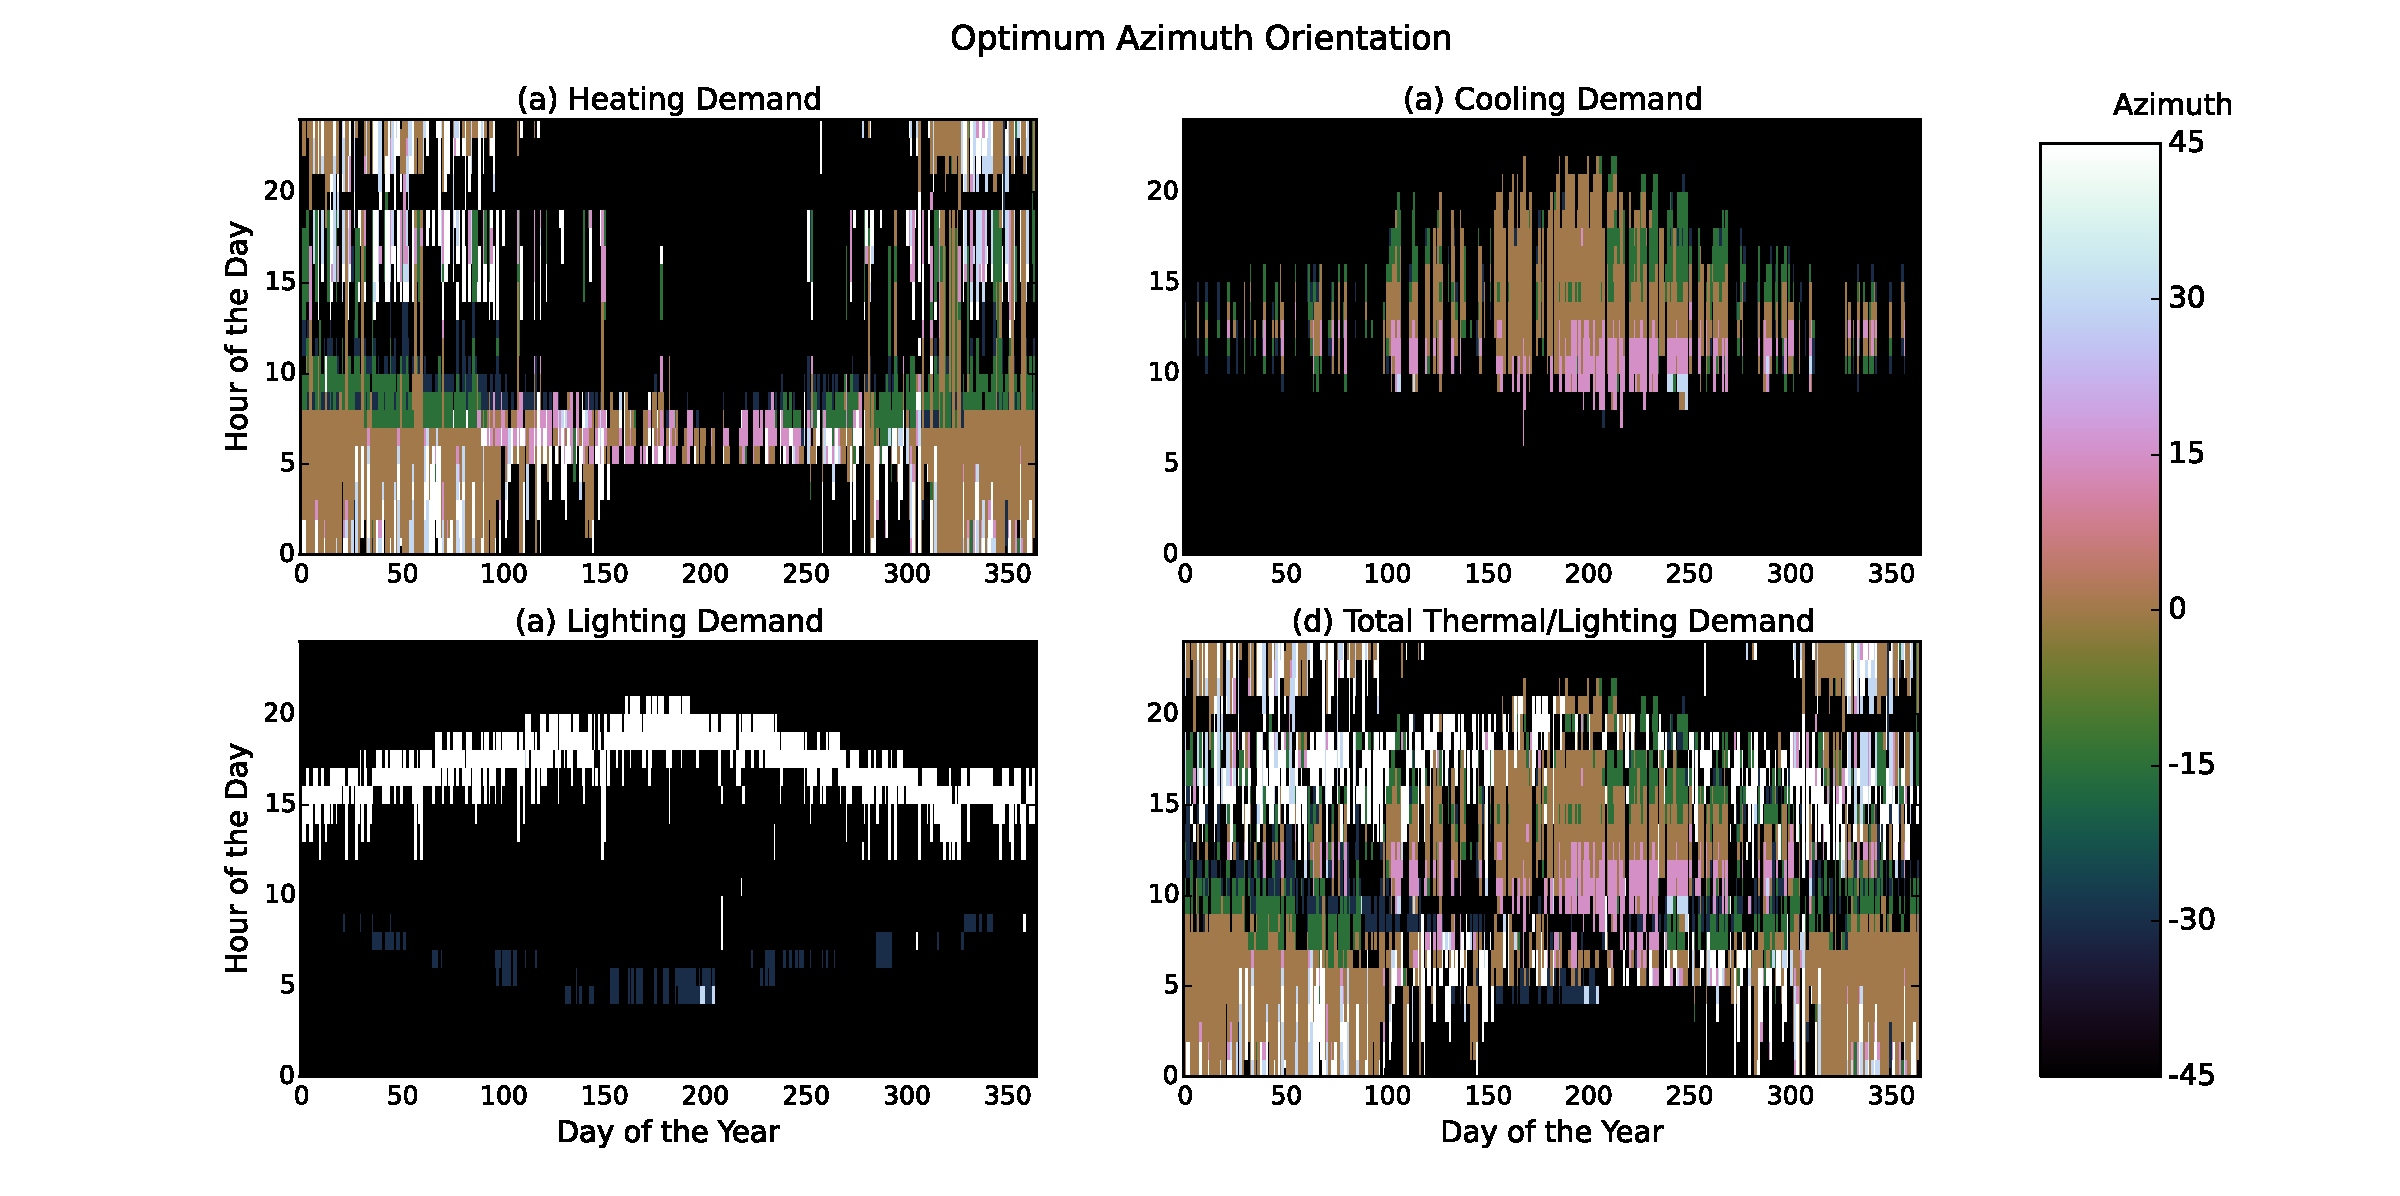
\includegraphics[width=\textwidth, trim= 0cm 0cm 0cm 0cm,clip]{DIVAy}
		\caption{Carpet plots detailing the optimal azimuth angles to minimise the (a) heating demand, (b) cooling demand, (c) lighting demand, and (d) total building energy demand. Cooling is minimized by bocking the sun, whereas lighting and heating is minimized by opening the facade to let the insolation in.}
		\label{f:DIVAy}
		\end{center}
	\end{figure*}

	Figure \ref{f:DIVAe} depicts the corresponding energy demand of the building for the whole year corresponding to the optimum positions presented in figures \ref{f:DIVAx} and \ref{f:DIVAy}. It can be seen that the heating heating is most needed during the winter and in the morning, whereas cooling is mainly apparent in summer afternoons. Lighting on the other hand is most important in the evenings and at times where there is not much sun. In the combined plot, this behavior be seen clearly as well, the main overlaps of different building energy consumptions take place during winter between heating and lighting in the morning and in the evening, and between cooling and lighting during summer evenings. 

	\begin{figure*}
		\begin{center}
		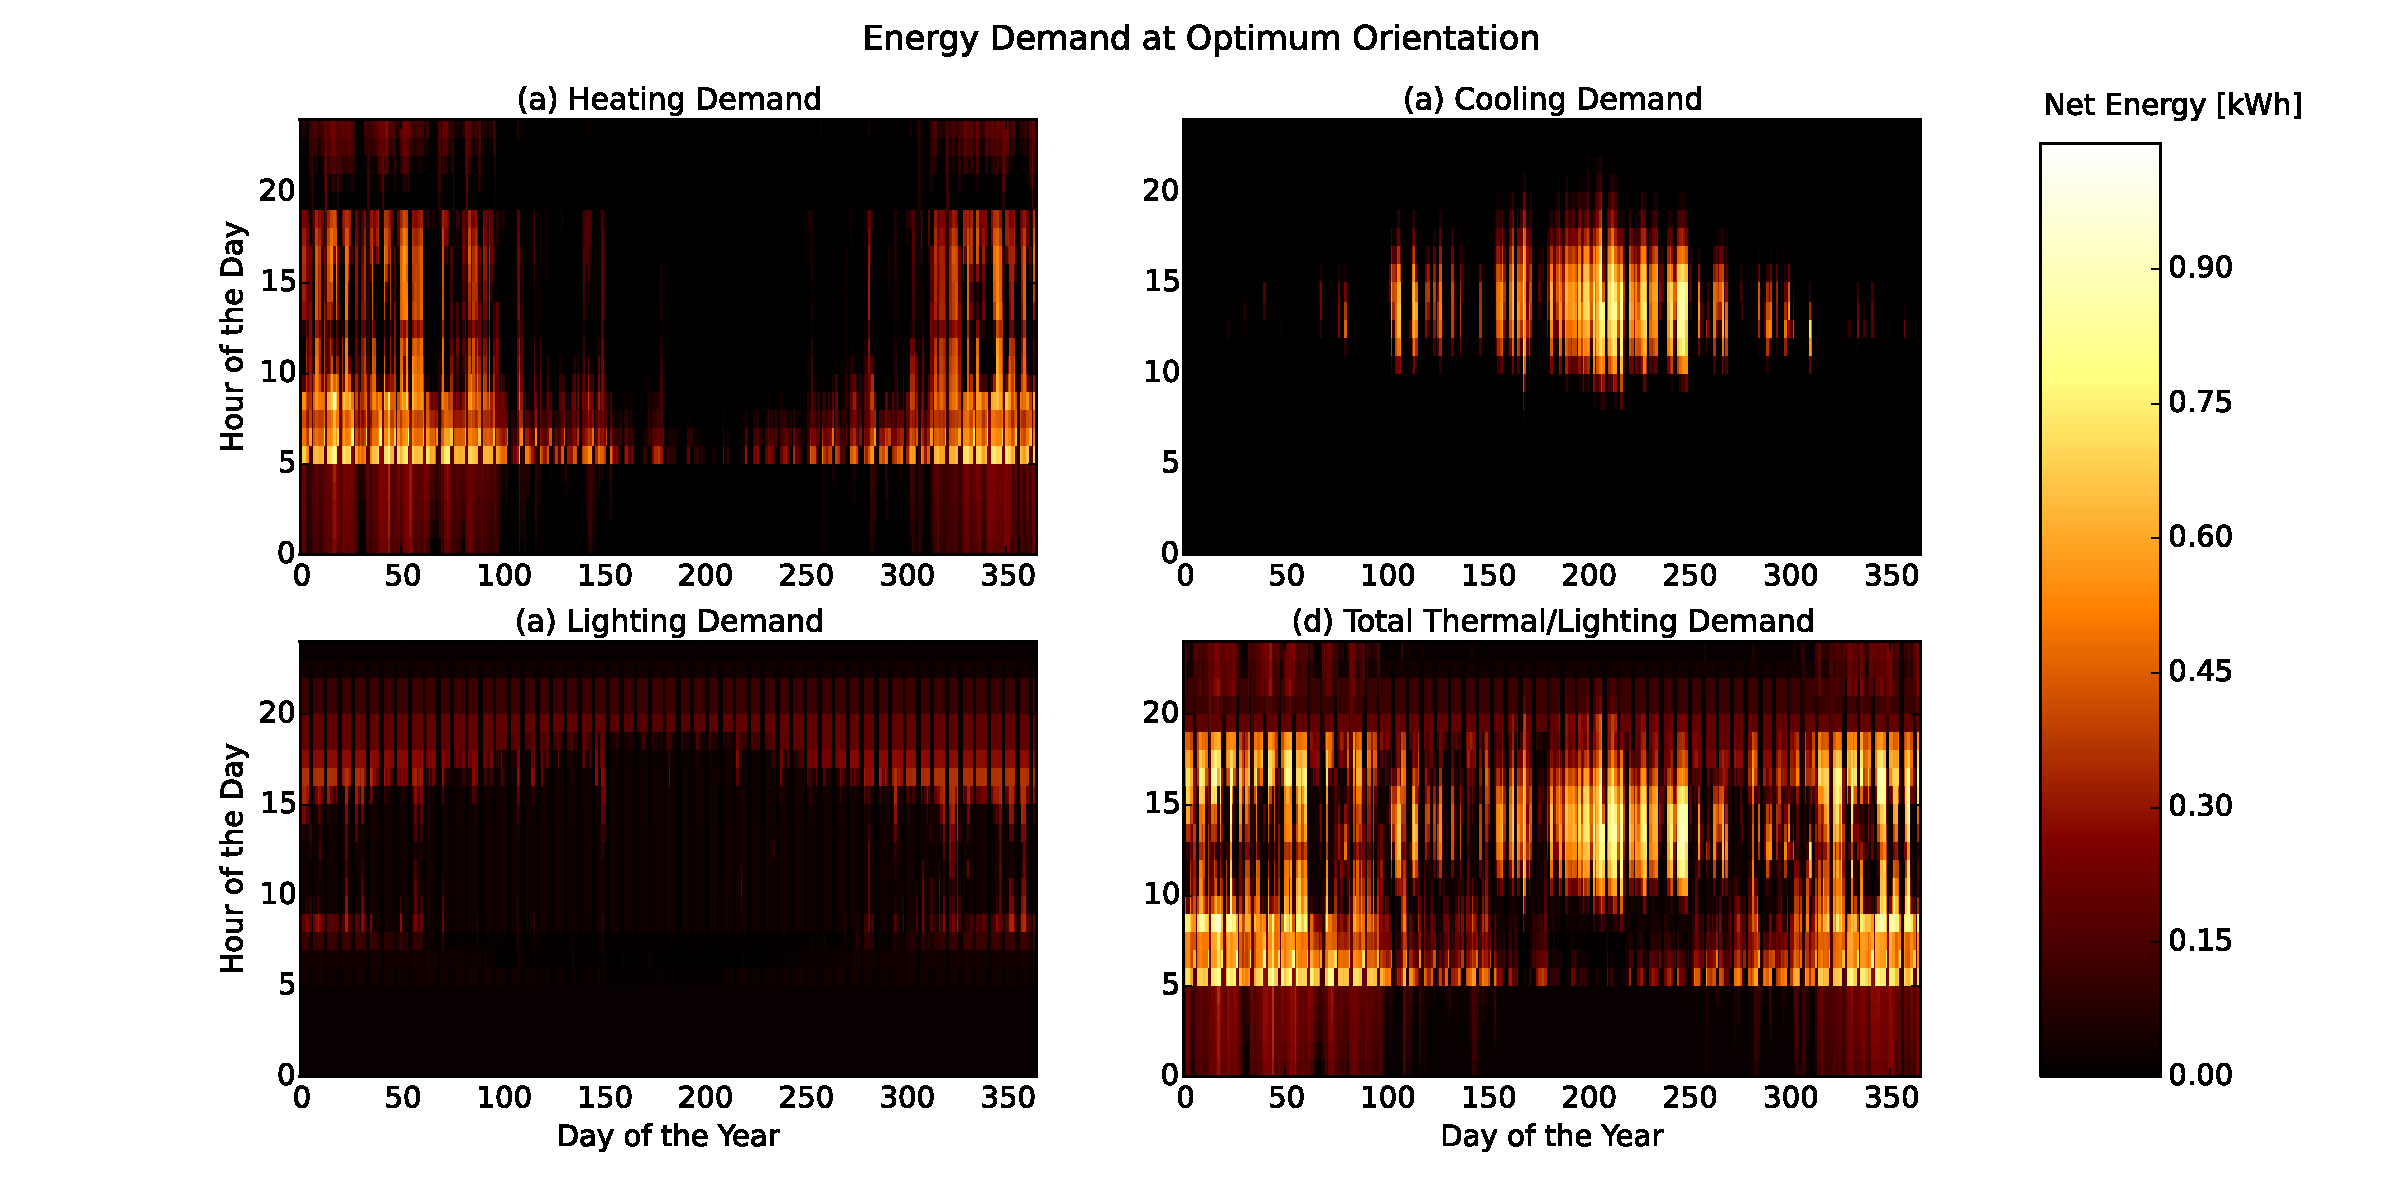
\includegraphics[width=\textwidth, trim= 0cm 0cm 0cm 0cm,clip]{DIVAe}
		\caption{Carpet plots detailing the net energy consumption. Each square represents the total energy consumption for that specific hour of the entire month. Red colours detail the energy demand, while blue colours detail the energy supply.}
		\label{f:DIVAe}
		\end{center}
	\end{figure*}
	
\section{Radiation and PV Analysis}
	
	To evaluate the performance of the radiation simulation, a grid-convergence study was performed and the optimum grid size for further simulations was found. The radiation results could then be used to calculate the PV electricity production, enabling the finding of optimum angles to maximize PV electricity production. The corresponding energy output was finally compared to a control strategy using solar tracking.

	\subsection{Grid Convergence}

		With a larger grid-size, results are less accurate. In order to study this effect, a grid convergence study was conducted. Figure \ref{f:gridConvergence} shows the grid size dependency of the total radiation on the asf. The colors in the first two plots on the upper left represent the hours of the day. One can see in the second plot - where the radiation is normalized by a division with the radiation for a grid-size of 12.5\,mm - that the results are significantly more accurate for morning and evening hours. This is caused by increased self-shading at midday hours. The colours in the third plot on the left show the dependency on different combinations. No clear pattern could be found here. Finally the average deviation is depicted in the fourth plot on the left and a box-plot with all deviations is shown on the right. It can be seen that a smaller grid-size leads to larger deviations. While for a grid-size of 400\,mm the average deviation is over 10\%, the deviation goes down to below 1\% for a grid size of 25\,mm. 25\,mm was therefore taken as the grid-size of all simulations, as it gives accurate results, while still being computationally feasible. 

		\begin{figure*}
			\begin{center}
			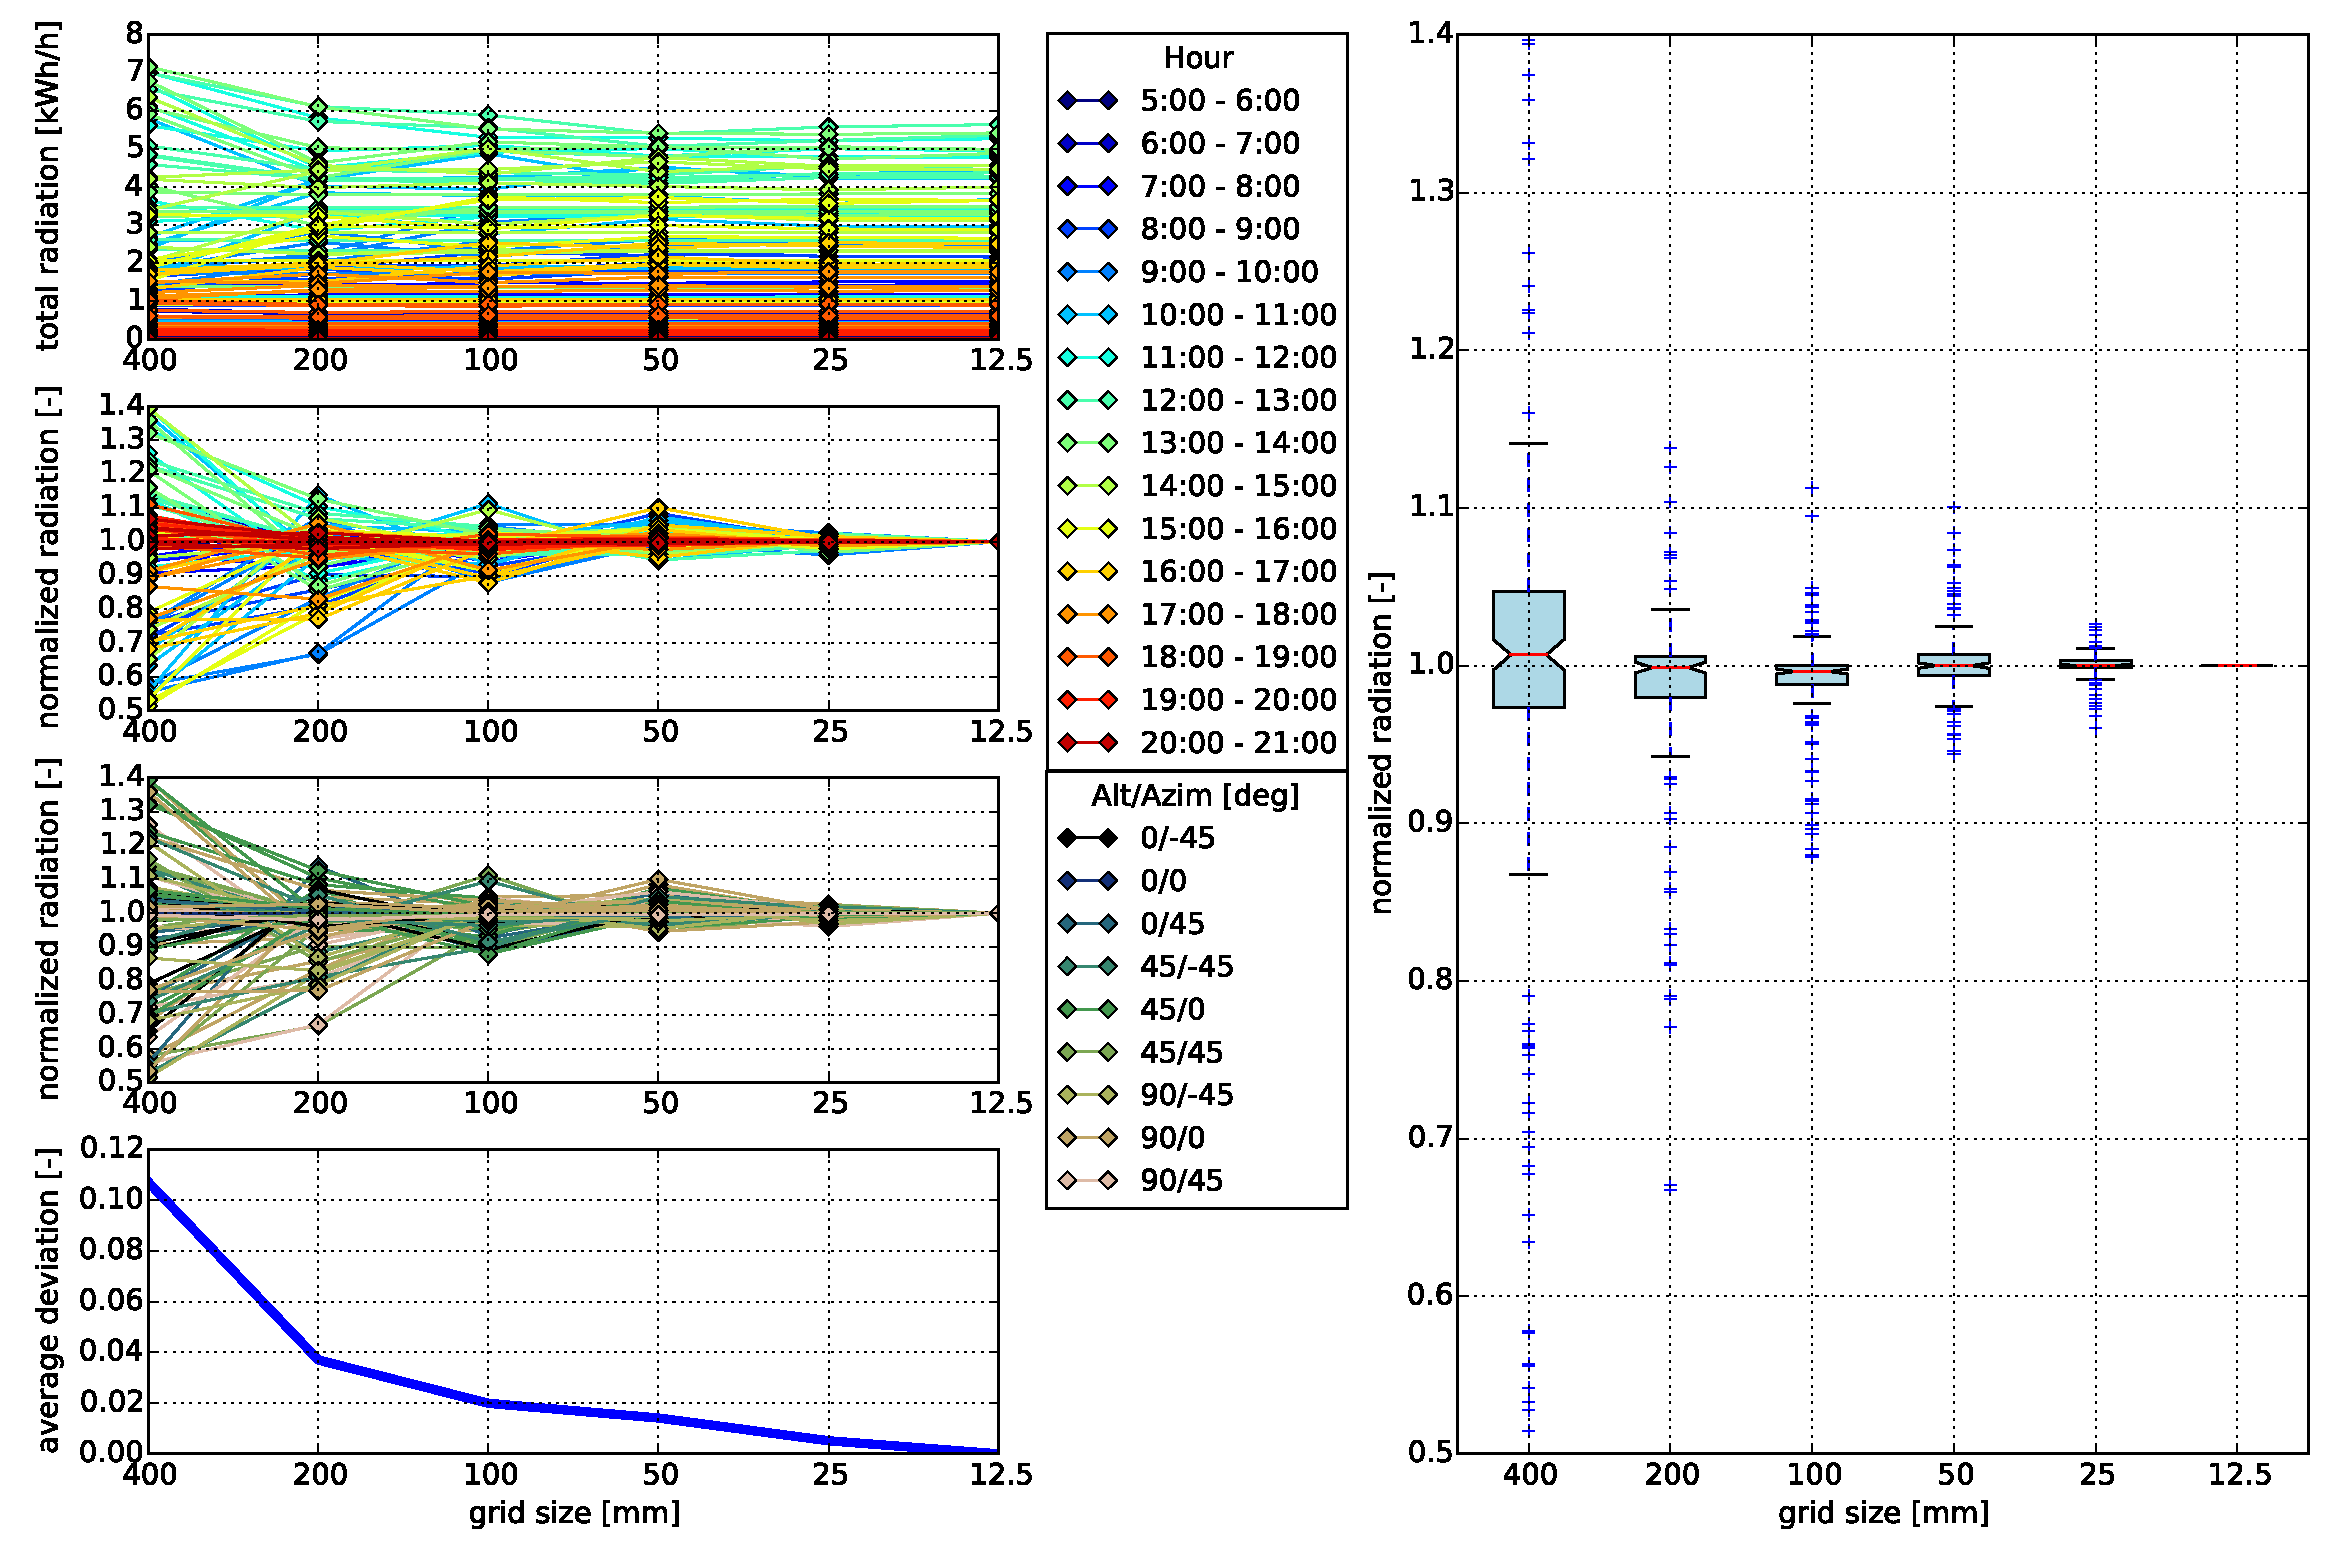
\includegraphics[width=\textwidth, trim= 0cm 0cm 0cm 0cm,clip]{gridConvergence.pdf}
			\caption{Grid convergence evaluation}
			\label{f:gridConvergence}
			\end{center}
		\end{figure*}

	\subsection{Comparison of Sun Tracking to Optimized Solution}

		In order to evaluate the optimum configuration for PV production, simulations using sun-tracking were compared to simulations evaluating the basecase of 49 different combinations (i.e. 7 different azimuth and altitude angles). In figure \ref{f:compareSuntracking} it can be seen that while the radiation on the panels is pretty similar for both sun tracking and the optimized solution, the PV electricity production of the optimized solution is significantly higher than the sun-tracking solution in the afternoon hours. This is caused by the layout of the PV panels, longitudinal shading causes high power losses \cite{hofer2015PVSEC}, thus the optimized solution decreases the longitudinal shading compared to sun-tracking. 

		\begin{figure*}
			\begin{center}
			\includegraphics[width=\textwidth, trim= 0cm 0cm 0cm 0cm,clip]{compareSuntracking}
			\caption{Comparison of optimized solution to sun-tracking. a) average radiation on panels compared to radiation without shading b) PV electricity production comparison c) efficiency comparison}
			\label{f:compareSuntracking}
			\end{center}
		\end{figure*}




\section{Combined Evaluation}

	By combining results for building energy simulations and PV electricity production, the overall optimum configurations can be found. Figure \ref{fig:carpetplot} details carpet-plots of the facade optimised to maximise PV generation, and minimise heating, cooling and lighting demands independently. It can be see that open configurations (light coloured) are chosen to minimise the building heating demands during the winter months and early mornings of spring and autumn. Likewise closed configurations (dark colours) are the preferred solutions to minimise the cooling demand during the summer months. Lighting control is only apparent during the twilight hours where the facade prefers an open position to avoid the use of artificial lighting. The PV optimisation follows a solar tracking model for most hours and as far as the limited range of angles allows. This causes some issues during twilight summer hours as the actuator cannot physically align itself normal to the sunlight. 




	\begin{figure*}
	\begin{center}
	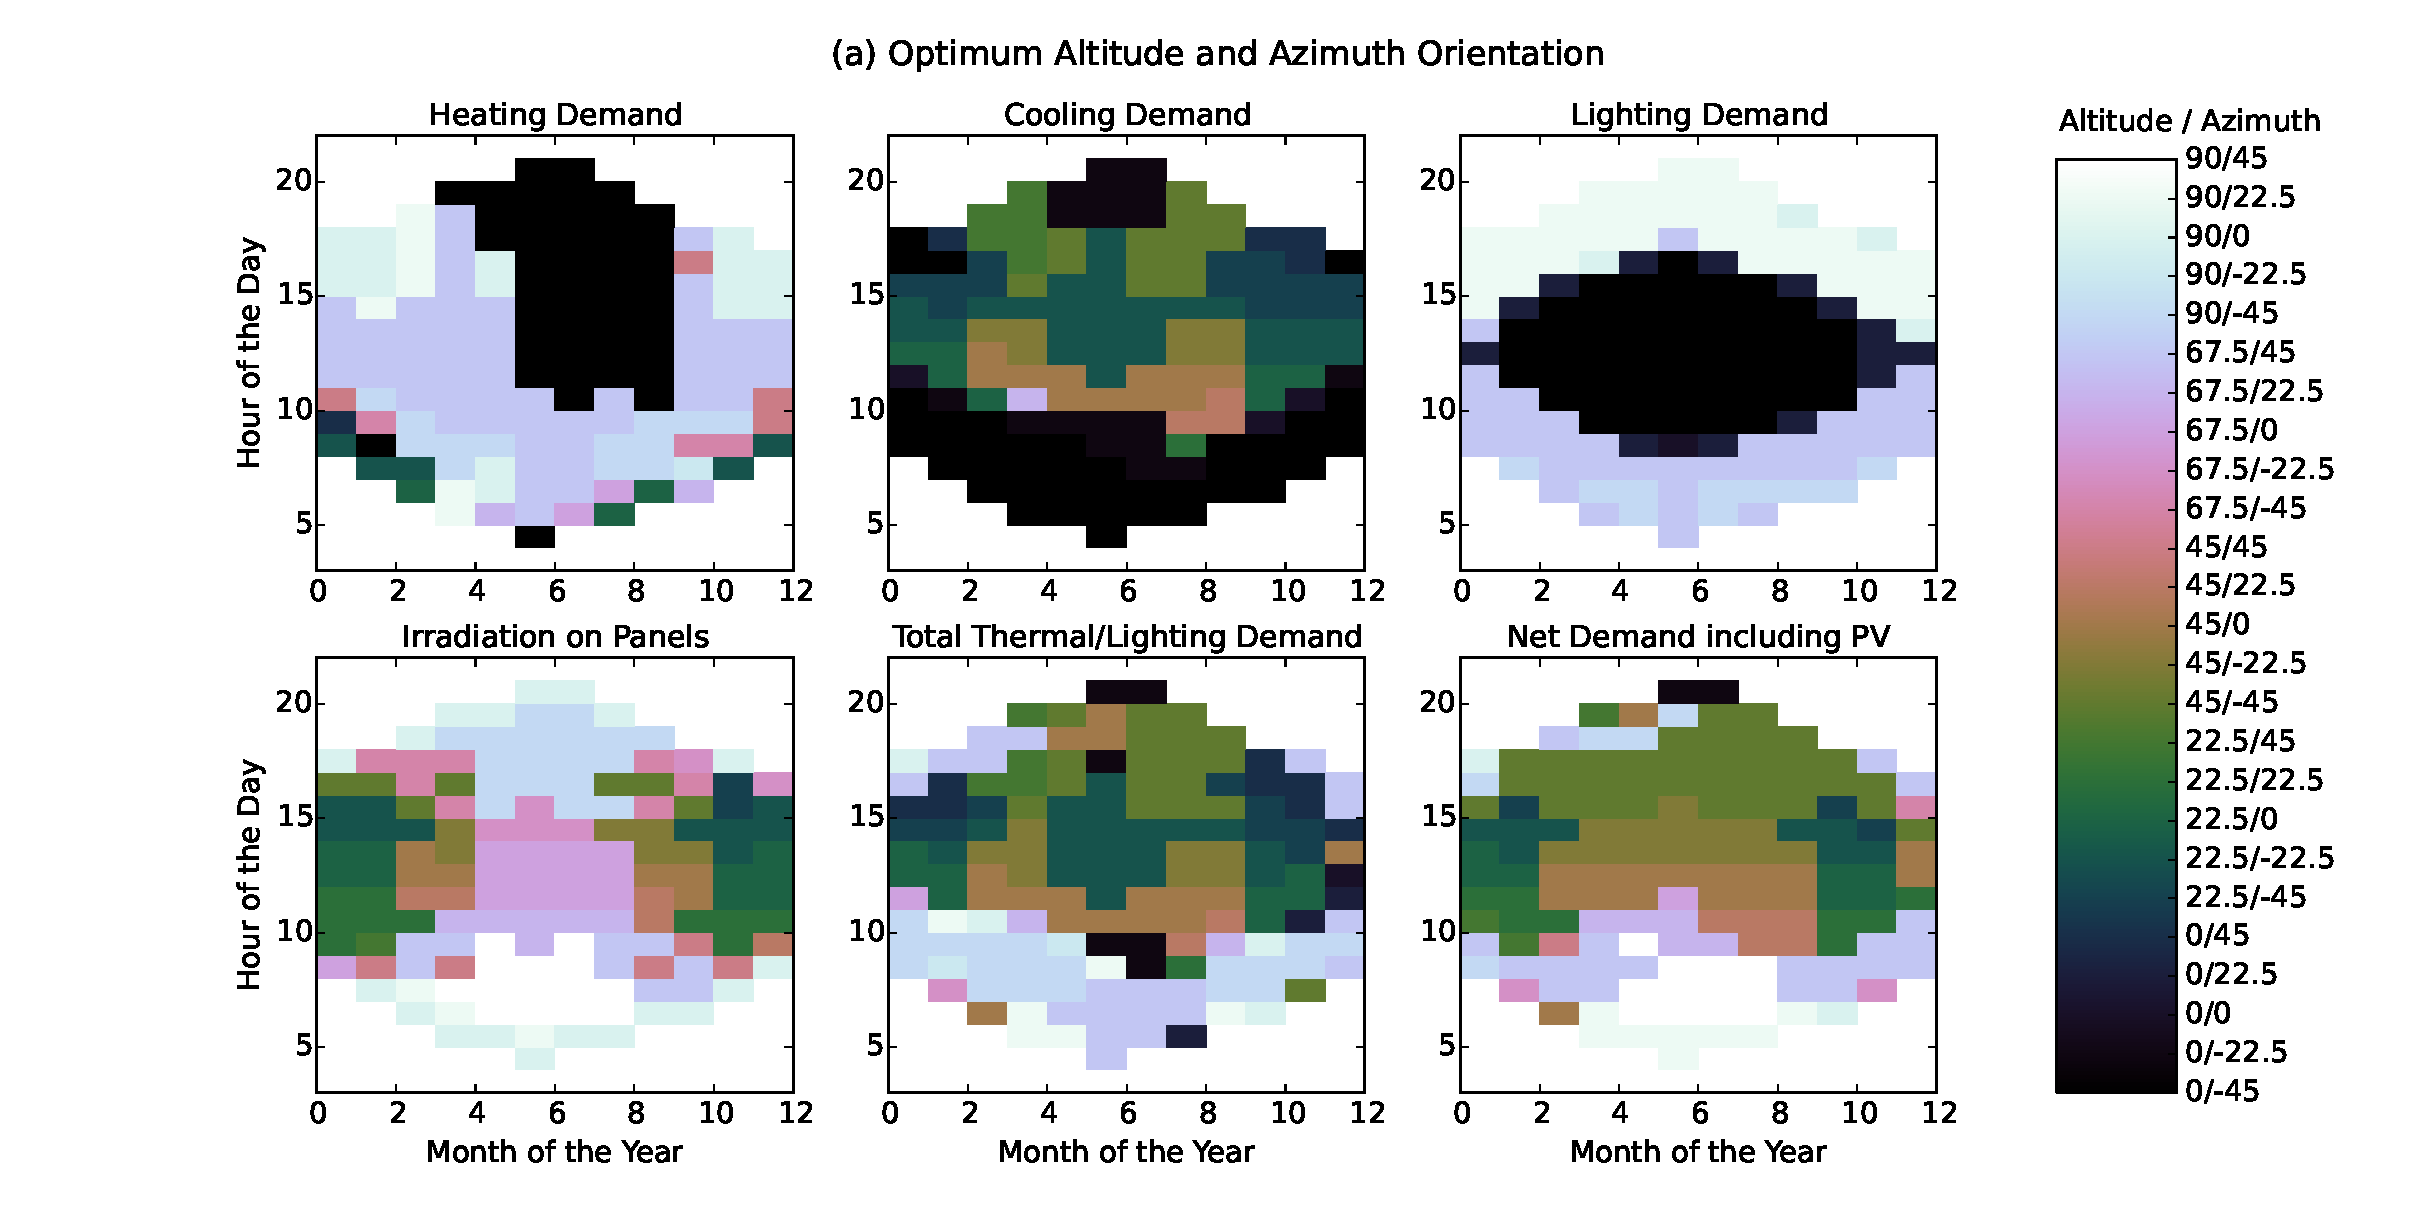
\includegraphics[width=\textwidth, trim= 0cm 0cm 0cm 0cm,clip]{carpetplot_angles.eps}
	\caption{Carpet plots detailing the optimal configuration to minimise the (a) heating demand, (b) cooling demand, (c) lighting demand, and (d) maximise irradiance on PV panels. Each configuration is represented by an angle of orientation around the x-axis (Altitude) and y-axis (Azimuth) as seen in the legend. Figure (e) details the combinations for optimum building thermal management without PV production. (f) also includes the PV production}
	\label{fig:carpetplot}
	\end{center}
	\end{figure*}

	\begin{figure*}
	\begin{center}
	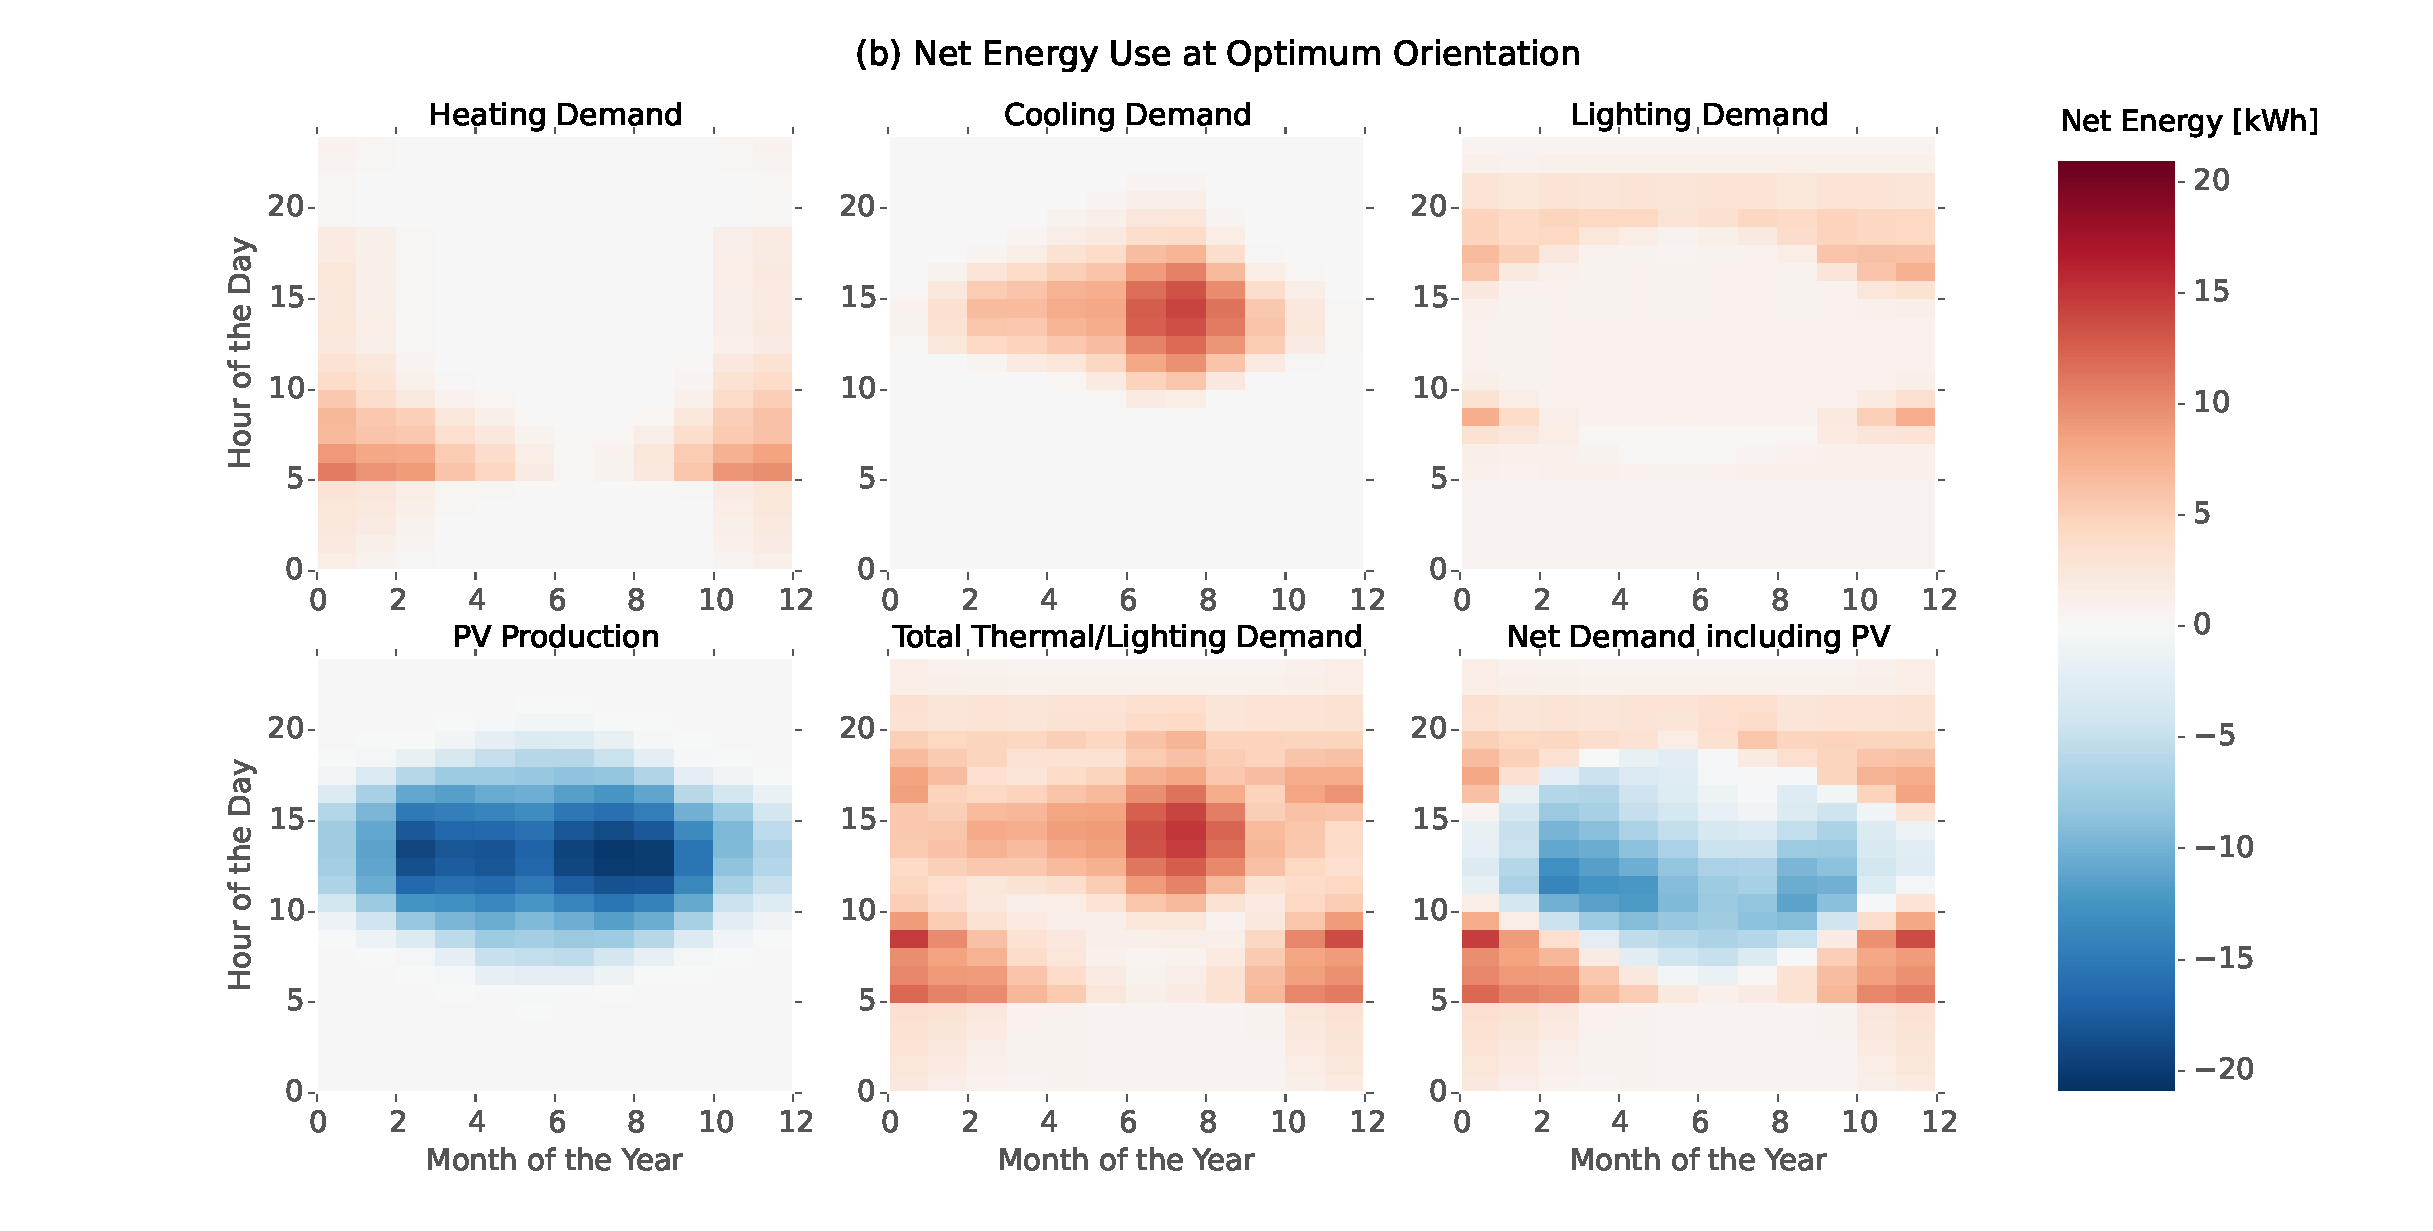
\includegraphics[width=\textwidth, trim= 0cm 0cm 0cm 0cm,clip]{carpetplot_energy.eps}
	\caption{Carpet plots detailing the net energy consumption. Each square represents the total energy consumption for that specific hour of the entire month. Red colours detail the energy demand, while blue colours detail the energy supply.}
	\label{fig:carpetplot_energy}
	\end{center}
	\end{figure*}



	When the four optimisation cases are combined to achieve the configurations for total energy minimisation we get some interesting results. There is a conflict in the summer evenings between minimising lighting and cooling demands. Likewise, we also see a conflict between heating and PV production during the winter months. The overall energy optimization including PV electricity production shows a strong tendency to follow the optimal PV production pattern. This, however changes if the building system becomes more inefficient. Less efficient heating for example, would result in configurations optimised for heating overpowering those of PV electricity generation.


	Figure \ref{fig:carpetplot_energy} shows the net energy use at these optimum angles. It is interesting to see how the combination of electricity generation and adaptive shading can compensate for the entire energy use during sunlit hours.

	\subsection{Orientation Analysis}

		Evaluations of the facade for different building orientations were done with the basecase of 5 azimuth and 5 altitude angles. Non suprisingly, the a south facing facade is produces the most electricity and has therefore the lowest net energy as can be seen in figure \ref{fig:buildingOrientation}. It was found that the PV apertures should be oriented parallel to the upper left edge for facades that are west or shouth-west oriented, whereas they should be oriented parallel to the upper right edge for east or south-east oriented facades. An east facing facade uses less heating compared to a west facing facade, as heating is most important during morning hours. For similar reasoning the east facing facade needs more cooling energy than the west facing facade, because the room heats up in the morning. Interestingly, PV production is higher for the west facing facade than for the east facing facade. The cause for this is probably because of confilcts in optimizing cooling and PV electricity production at the same time, as cooling is more dominant for the east facing facade. 

		\begin{figure*}
		\begin{center}
		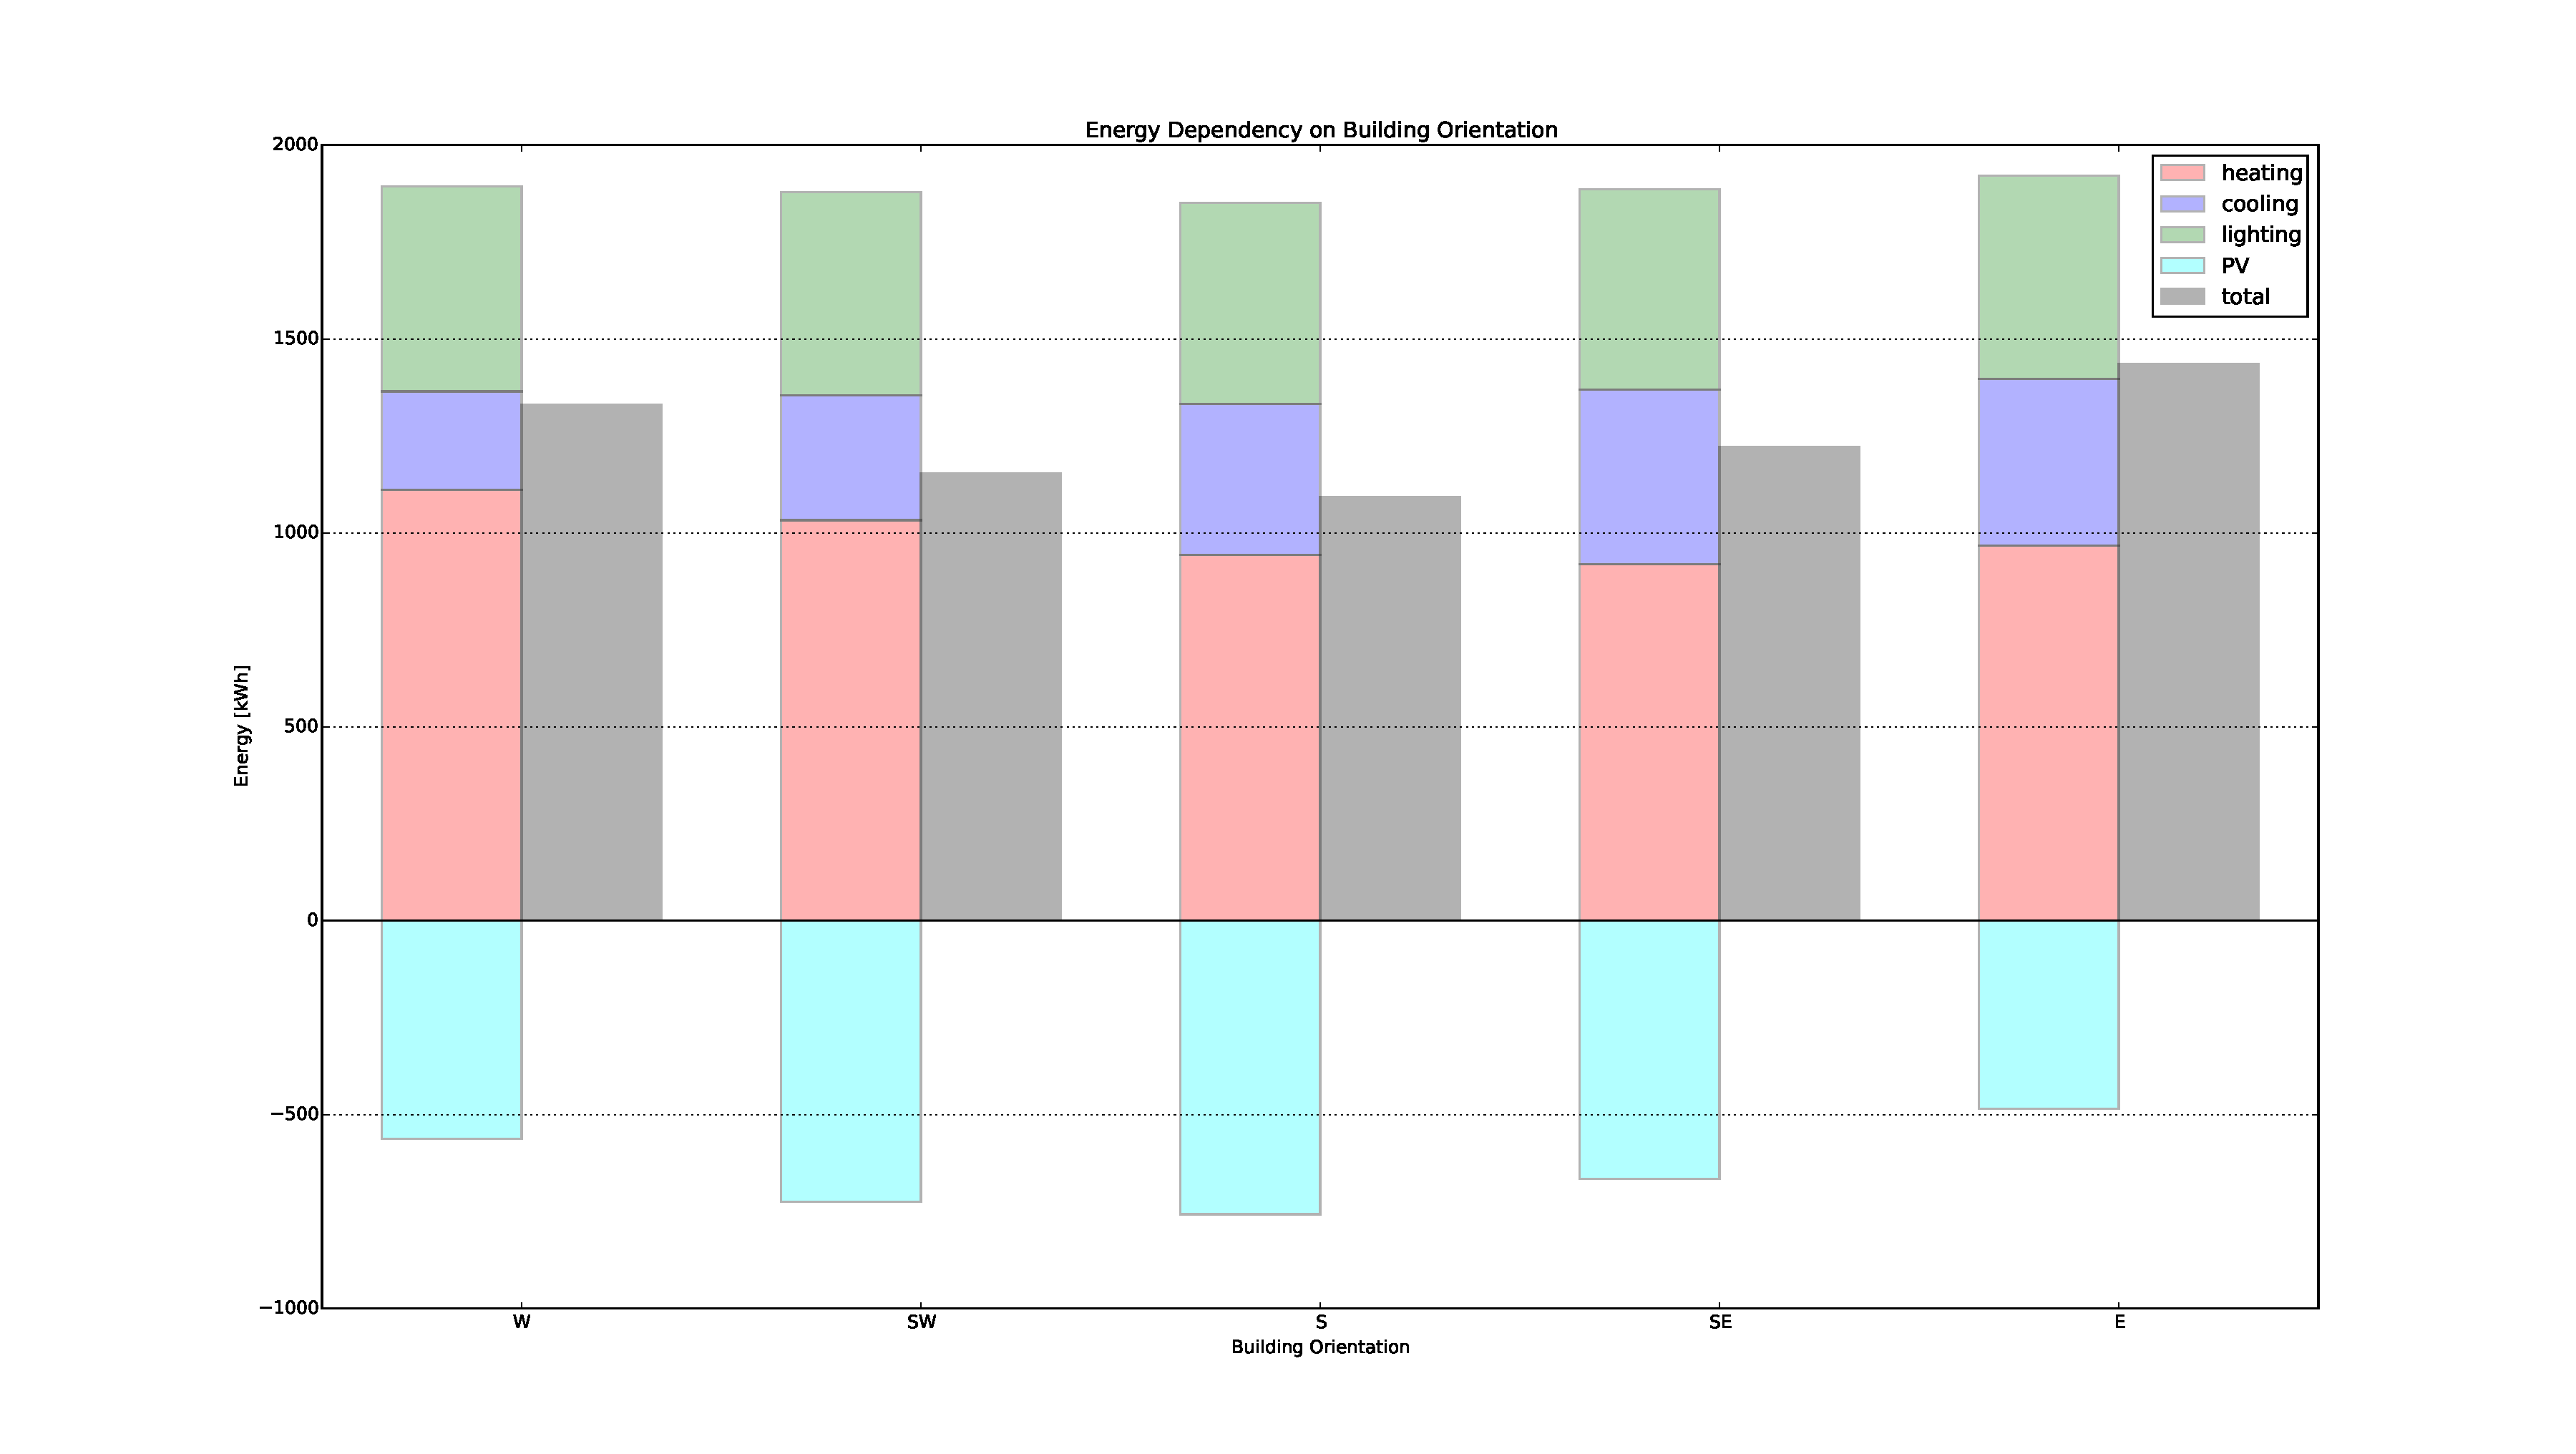
\includegraphics[width=\textwidth, trim= 0cm 0cm 0cm 0cm,clip]{buildingOrientation}
		\caption{Energy demand in dependence of building orientation. South facing facades perform best.}
		\label{fig:buildingOrientation}
		\end{center}
		\end{figure*}

	\subsection{Sensitivity Analysis}

		A sensitivity analysis was done for heating COP, cooling COP, lighting load, average PV efficiency, building orientation, infiltration rate and combination variations for the time period of one year. The results are shown in figure \ref{fig:sensitivity}. The top row shows the energy savings per square meter of room area compared to a fixed solare facade at an angle of 45\degree, whereas the bottom row shows the energy savings compared to a building without any pv modules or shading devices. 

		\begin{figure*}
		\begin{center}
		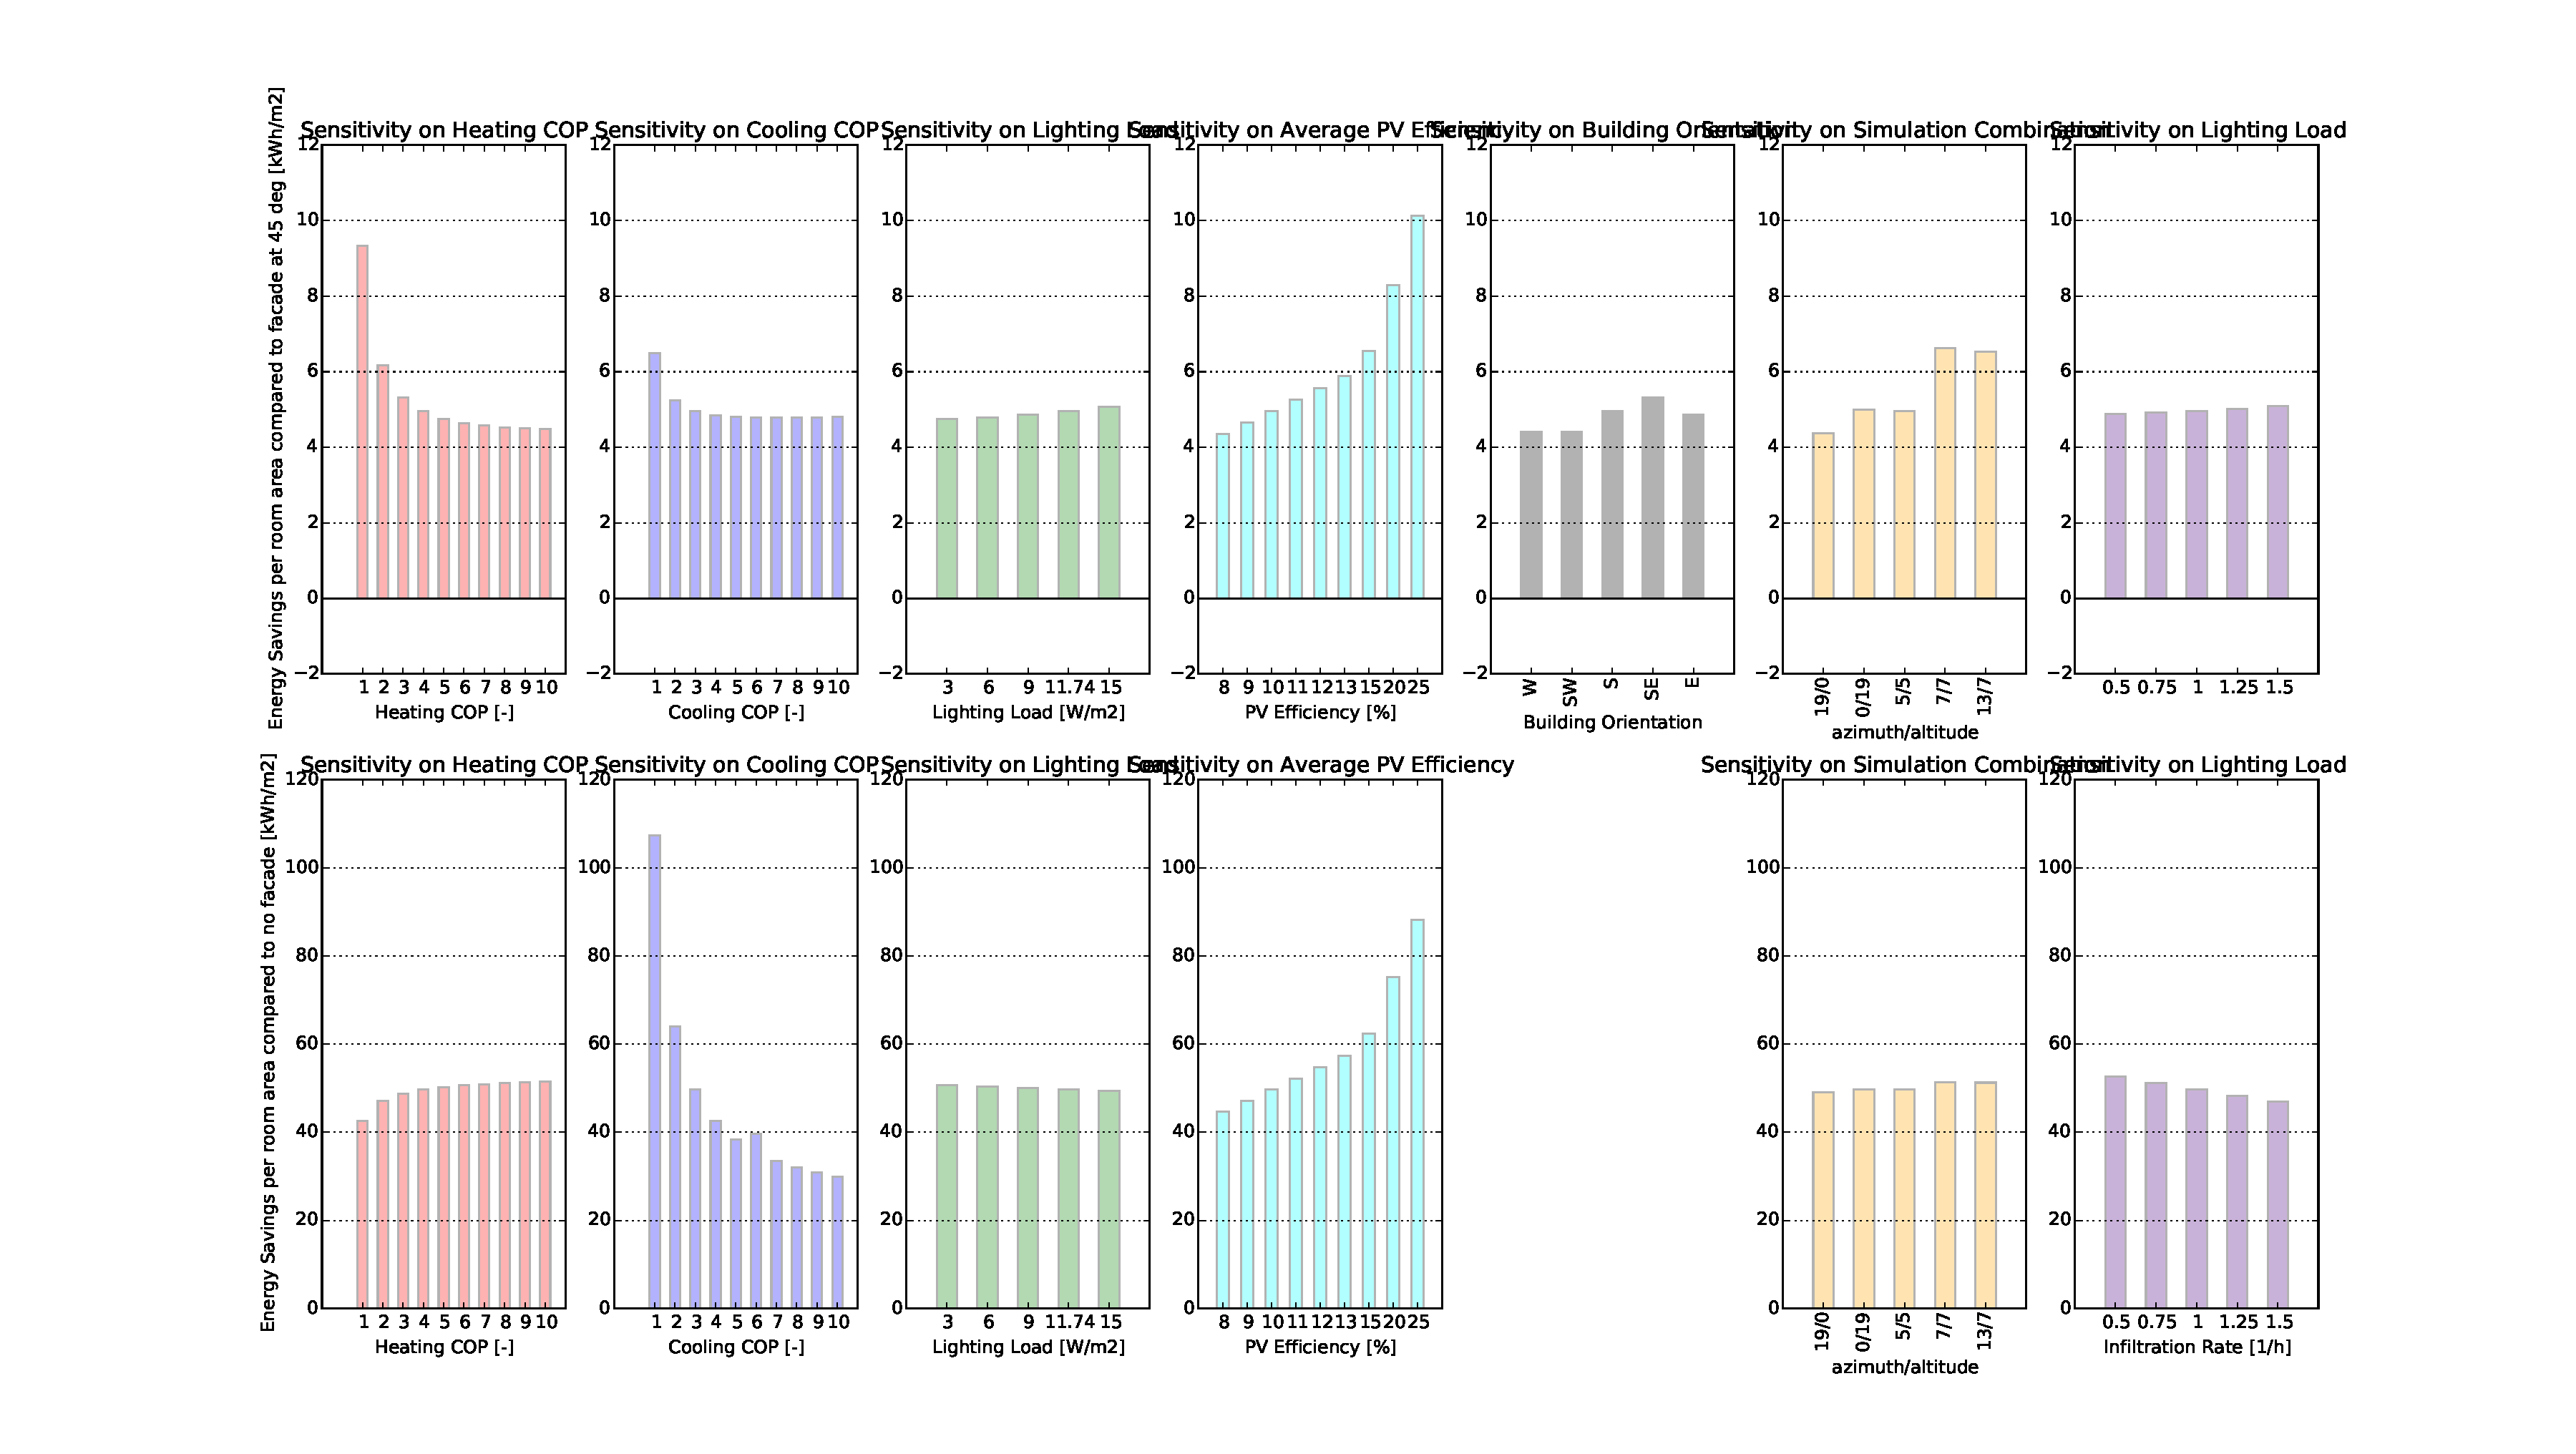
\includegraphics[width=\textwidth, trim= 0cm 0cm 0cm 0cm,clip]{sensitivity}
		\caption{Sensitivity analysis of energy savings during one year. From left to right, sensitivites on heating COP, cooling COP, lighting load, average PV efficiency, building orientation, combination variations and infiltration rate. Top row shows the energy savings compared to a fixed solar facade at a 45\degree altitude angle, the bottom row shows the energy savings compared to a room without shading or PV modules.}
		\label{fig:sensitivity}
		\end{center}
		\end{figure*}